\documentclass[12pt]{article}

% Packages
\usepackage{hyperref}
\usepackage[utf8]{inputenc}
\usepackage{graphicx}
\usepackage{color}
\usepackage{afterpage}
\usepackage[nottoc,numbib]{tocbibind}
\usepackage{amsmath}
\usepackage{tocloft}
\usepackage{array}
\usepackage{fancyhdr}
    \fancyfoot{}
    \lhead{Chelcea Claudiu, \thepage}
    \pagestyle{fancy}

% Author and project setup
\author{Chelcea Claudiu-Marian}
\title{Dezvoltarea de jocuri video - motoare grafice}
\date{03.18.2021}
\renewcommand{\contentsname}{Cuprins}
\renewcommand{\refname}{Bibliografie}
\setlength{\arrayrulewidth}{1mm}
\setlength{\tabcolsep}{18pt}
\renewcommand{\arraystretch}{1.5}
\addtocontents{toc}{\protect\enlargethispage{\baselineskip}}
\newcommand{\spaceto}[2]{{\ooalign{$\phantom{#1}$\cr\hidewidth$#2$\hidewidth}}}
\renewcommand\cftsecfont{\LARGE}
\renewcommand\cftsecpagefont{\LARGE}
\renewcommand{\figurename}{Fig.}

% Main code
\begin{document}

% Intro page
\begin{titlepage}
  \afterpage{\pagecolor{white}}%
  \LARGE
  \begin{center}
  \begin{figure}
  
\includegraphics[width=\linewidth]{UnrealUnity.jpg}
  \caption{Unity vs Unreal Engine,  imagine: \href{https://www.htlo.co.uk/unity-vs-unreal-engine-a-quick-comparison/}{HTLO}.}
  \label{fig:UvsUE}

\end{figure}

    {\bfseries Dezvoltarea de jocuri video - motoare grafice}\\[3em]
    {\large
      \begin{tabular}{rl}
      \textbf{Nume:} & Chelcea Claudiu-Marian \\
	\textbf{Universitate:} & Universitatea Politehnica din București \\
	\textbf{Facultate:} & Facultatea de Automatică și Calculatoare  \\
      \textbf{Specializarea} & Calculatoare și Tehnologia Informației  \\
	\textbf{Grupa:} & 312CA \\
 	\textbf{Data:} & 03.19.2021 
	
      \end{tabular}%
    }
  \end{center}
\end{titlepage}

% Contents page
\newpage
\tableofcontents

% First page
\newpage
\section{De ce un motor grafic?}
\hspace{10pt}
Un motor grafic este un sistem conceput pentru crearea și dezvoltarea de {\it jocuri video}. \par Există mai multe motoare de joc, care sunt proiectate să funcționeze pe console de jocuri video și calculatoare personale. 
\par Funcționalitatea de bază oferită de obicei de un motor grafic include un motor de randare (engleză "renderer") pentru grafică {\bf 2D} sau {\bf 3D}, un motor de fizică sau de detectare a coliziunilor (și răspunsul la coliziune), sunet, scripting, animație, inteligență artificială, rețea, streaming, memorie de management, suport de localizare, etc. \par Procesul de dezvoltare a jocului este de multe ori economisit, în mare parte, prin reutilizarea / adaptarea unui motor asemănător pentru a crea jocuri diferite.
\subsection
{\bf Avantaje:}
\begin {itemize}
\item Majoritatea, dacă nu tot codul poate fi generat de aplicație, deci va puteți ocupă doar de aspect, logică.
\item În această direcție, gestionarea memoriei, încărcarea sprite-urilor, iluminarea (în motoare complexe) etc. au fost proiectate și testate temeinic.
\item Dacă motorul este capabil de "multiplatform", portabiltiatea către alte platforme va fi ușurată semnificativ.
\end{itemize}

\subsection
{\bf Dezavantaje:}
\begin {itemize}
\item Dacă există o eroare în motor, dacă nu este open source, nu o puteți remedia.
\item Motorul nu a fost conceput special pentru jocul dvs., deci poate fi mai puțin eficient decât codul pe care îl scrieți special pentru acesta.
\item Motoarele de joc nu sunt, în general, gratuite.  \footnote[2]{Puteți citi mai multe la https://gamedev.stackexchange.com/questions/859/what-are-the-advantages-and-disadvantages-to-using-a-game-engine.}
\end{itemize}

% Second page
\newpage
\section{Ce motoare grafice sunt populare?}
Pentru crearea unui joc la scala mică, este recomandat să se folosească un limbaj de programare, pentru a obține performanța maximă. Pentu lansarea unui joc de dimensiune medie, care poate fi vândut către alți oameni, este recomandat să se folosească un motor grafic, deoarece ușurează implementarea functionalitatilor de baza și, în cele mai multe cazuri, acestea sunt mai performante decât codul scris manual, întrucât au fost testate și optimizate constant până au fost introduse în aplicație.\\

Studio-urile de jocuri, în general, combină aceste două moduri de a crea un joc, implementând logica jocului prin Visual Scripting sau alte facilități oferite de motorul grafic folosit, adăugând propriile funcționalități prin cod, în general C++, iar, în cazuri rare, Csharp, Python, Java.\\
\hspace{5pt}\\ Lista {\bf celor mai populare 8} motoare grafice, conform \href{https://www.gamedesigning.org/career/video-game-engines/}{GAMEDESIGNING}:\footnote[1]{Aceste statistici sunt actuale la data de 19 Martie 2021.} 
\begin{enumerate}
  \item Unreal Engine.
  \item Unity
  \item GameMaker
  \item Godot
  \item AppGameKit
  \item CryEngine
  \item Amazon Lumberyard
  \item RPG MAKER \\
\end{enumerate}


O analiză de la Gamasutra a constatat că {\bf Unreal Engine} și {\bf Unity} sunt printre cele mai populare motoare de joc. Această analiză s-a bazat pe jocuri lansate pe Steam și Itch.io.

% Third page
\newpage
\section{Diferen\c{t}e dintre Unity si Unreal Engine}
Răspunsul la care este mai bun este o chestiune dificilă. Unii vor susține că Unreal este mai bun doar pentru faptul că este o alegere de top pentru studiourile AAA. Cu toate acestea, alții vor cita faptul că Unity este mai bine rotunjită și, pentru dezvoltatorii independenți, este adesea o intrare mai bună în industrie. Obiectiv, însă, este unul mai bun decât celălalt?

\subsection{Unity}
Unity este frecvent utilizată deoarece este:
\begin{itemize}
\item O platformă de creare 3D deschisă și avansată în timp real.
\item Folosit pentru a produce jocuri în mai multe genuri.
\item Integrat cu instrumente cheie de dezvoltare a jocurilor, inclusiv IDE-uri, instrumente grafice și controlul versiunilor.
\end{itemize}

\subsection{Unreal Engine}
Unreal Engine este frecvent utilizat deoarece este:
\begin{itemize}
\item Un motor de joc multiplataforma, cu suport pentru peste 25 de platforme.
\item O platformă de dezvoltare 3D în timp real.
\item Integrat cu instrumente cheie de dezvoltare a jocurilor, inclusiv IDE-uri, instrumente grafice și controlul versiunilor.
\end{itemize}

De ce e util să folosim un motor grafic?
În caz că nu folosim un motor grafic, o să folosim formule de tipul următor pentru un simplu shader asupra oceanului: \footnote[3]{Autor necunoscut al formulei} \\
 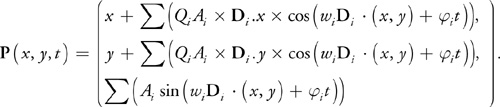
\includegraphics[width=\linewidth]{water.jpg}

% Fourth page
\newpage
\section{Grafica pe calculator = matematică}
\subsection{Shader pentru lumină}
Efectul de estompare al luminilor punctiforme se numește de obicei atenuare. Atenuarea unei lumini reale este guvernată de legea pătratului invers care spune că puterea luminii este invers proporțională cu pătratul distanței de la sursa de lumină. Aceasta este descrisă în termeni matematici prin următoarea formulă:

$$ L_{distance} = \frac{L_1}{distance^2}   \hspace{25pt}    (L_1    \hspace{10pt}este \hspace{10pt}    intensitatea    \hspace{10pt} luminii) $$

Această formulă nu oferă rezultate bune în grafica 3D. De exemplu, pe măsură ce distanța devine mai mică, puterea luminii se apropie de infinit. În plus, dezvoltatorul nu are control asupra rezultatelor, cu excepția setării puterii inițiale a luminii. Acest lucru este prea limitativ. Prin urmare, se adaugă câțiva factori la formulă pentru a o face mai flexibilă:

$$ L_{distance} = \frac{L_1}{Atenuare_{constanta} + Atenuare_{liniara} * distanta + Atenuare_{exponentiala} * distanta^2} $$

\subsection{Shader pentru sticlă si metal}
În shader-ul de metal și sticlă, vom utiliza aproximarea Schlick pentru a calcula reflectanța F și transmitanța T. Reflectanța (sau coeficientul de reflecție) este fracțiunea de lumină care se reflectă, iar transmitanța (sau coeficientul de transmisie) este fracțiune de lumină care este refractată. Sub modelul nostru, toată lumina este fie reflectată, fie transmisă, deci $ T + F = 1. $ \\ \\
Teta este unghiul dintre suprafața normală și vectorul de la cameră la vârful i.
R este reflectanța la incidență normală (adică fracția de lumină reflectată atunci când $ Teta_i $ este zero). Este o constantă care va fi transmisă în umbră
Determinăm F prin aproximarea lui Schlick după cum urmează:
\begin{equation} 
 F \approx R_0 + (1 - R_0)(1 - cos\theta_i)^5
\end{equation}

% Fifth page
\newpage
Modelul de iluminare Phong: \\
Modelele de iluminare Phong și Blinn-Phong au fost primele modele de iluminare încercate mimând fenomene de reflexie speculară. Cu toate acestea, aceste modele nu se bazează pe realitate pentru că modelul Phong împarte iluminatul în trei termeni diferiți: ambient, difuz și specular.
Conform modelului Phong:
\begin{equation}
 k_{spec} = \cos^n(E,  R) 
\end{equation}
unde n este coeficientul specular, E indică în direcția vizualizatorului, iar R este  reflectarea vectorului luminii primite despre vectorul normal.
Valorile mai mari ale n produc momente speculare mai luminoase, mai localizate. \\

{\bf Un model mai bun de iluminare: Cook-Torrance.} \\
Există multe alte tehnici de iluminare care modelează mai bine distribuția microfacetelor (avioane plate foarte mici) care alcătuiesc o suprafață. Una dintre acestea este cea bazată fizic Modelul Cook-Torrance, utilizat în stocul PBR shader într-o serie de aplicații populare de creare 3D (inclusiv Blender). Veți folosi acest model pentru a calcula termenul specular. În special,
$$ k_{spec} = \frac{DFG}{V * N} $$
unde D = factorul de distribuție Beckmann: $$ D = \frac{exp(-\tan^2(\alpha)/m^2)}{4m^2\cos^4(\alpha)}, $$ \\ $ \alpha = arccos{(n * h)}, $
F este coeficientul Fresnel (calculat folosinde aproximarea lui Schlick), iar G este geometric termen de atenuare cauzat de auto-umbrirea microfacetelor de la suprafață,

% Sixth page
\newpage
\section{Înapoi la motoare grafice}
Am observat că construirea proprie a shader-lor este o muncă foarte dificilă și necesită foarte multe cunoștințe de matematică și fizică.

Pentru a face lucrurile mai ușoare, un dezvoltator de jocuri începător va folosi întotdeauna un motor grafic. Din statistici \footnote[4]{Statistici: https://www.perforce.com/blog/vcs/most-popular-game-engines}\footnote[5]{Statistici: https://www.gamedesigning.org/career/video-game-engines/}\footnote[6]{Statistici: https://gamedevacademy.org/best-game-engines/} a reieșit că {\bf Unity} a reieșit că {\bf Unity} și {\bf Unreal Engine} sunt cele mai utilizate motoare grafice, așa că, care este diferența dintre ele? \\ \\
\begin{tabular}{c|c|c}
    Topic & Unity & Unreal Engine \\ \hline
    Preț & \text{Gratuit și 5\% din profit} &\text{Gratuit și 5\% din profit}\\ 
    Interfață & Ușor-Medium & Greu \\
    Resurse disponibile & Foarte multe & Limitate  \\ 
    Dezvoltate jocuri & Programare C\#  & Programare C++ \\ 
    Grafică & Medie & Foarte bună  \\ \\
\end{tabular}

\subsection{Concluzie:}
\hspace{15pt} Alegerea unui motor grafic pentru realizarea unui joc este foarte importantă și este făcută, în special, în funcție de tipul de joc dorit. \\

Astfel, pentru realizarea jocurilor 2D - platformer, 2.5D sau jocuri pentru telefon, jocuri care nu necesită cea mai mare atenție la detaliile grafice, este preferat motorul Unity, pentru rapiditatea pe care o oferă în dezvoltarea jocurilor video. \\

Pentru realizarea jocurilor 3D, cu predilecție a jocurilor AAA, este utilizat Unreal Engine, datorită tuturor functionalitatilor pe care le oferă, sau, în caz contrar, se utilizează un motor grafic dezvoltat de către companie, denumite motoare 'în-house'.



% Bibliography
\newpage
\begin{thebibliography}{}
\bibitem{text1} 
\href{https://ro.wikipedia.org/wiki/Motor_grafic}{Wikipedia: motor grafic link}
\bibitem{text1} 
\href{https://www.gamedesigning.org/career/video-game-engines/}{Gamedesigning: website link}
\bibitem{text1} 
\href{https://www.gamasutra.com/}{Gamasutra: website link}
\bibitem{text1}
\href{https://www.htlo.co.uk/unity-vs-unreal-engine-a-quick-comparison/}{HTLO: website link}
\bibitem{text1}
\href{https://gamedevacademy.org/unity-vs-unreal/}{GameDev Academy: website link}
\bibitem{text1}
\href{http://ogldev.atspace.co.uk/www/tutorial20/tutorial20.html}{Sursa formulei shader-ului de lumină}
\bibitem{text1}
\href{https://cs.brown.edu/courses/cs123/labs/lab09.pdf}{Sursa formulei shader-ului de sticlă si metal}
\end{thebibliography}

\end{document}
